\section{Tensor Derivatives: levelling up the rizz!}
Till now, we had just seen the transformation of tensors and tensor densities. However, an important aspect of any calculation is the ability to take derivatives \footnote{A person's intellectual prowess can be judged their ability to take derivatives \emoji{smiling-face-with-sunglasses}}. Derivatives occur everywhere in calculations and we need a way to tackle them. So let's start\dots

\subsection{Velocity}
Well velocity is a vector (we had been reminded many a times) and it should then transform as a vector. Now, 
we know the transformation:
$$dx'^i = \pdv{x'^i}{x^l}x^l$$
To find velocity components, we have to differentiate with respect to time $t$. 
\begin{align*}
    \dv{x'^i}{t} &= \dv{\pdv{x'^i}{x^l}x^l}{dt}\\
    &=\pdv{x'^i}{x^l}\dv{x^l}{t} + x^l \dv{\pdv{x'^i}{x^l}}{t}\\
    &=\pdv{x'^i}{x^l}\dv{x^l}{t} + x^l \pdv{x'^i}{x^k}{x^l}\dv{x^k}{t}
\end{align*}
Now we define $v^k = \dv{x^k}{t}$. Then the above expression would give:
\begin{align*}
    v'^k = \pdv{x'^i}{x^l}v^l +  \pdv{x'^i}{x^k}{x^l}x^l v^k
\end{align*}
The first term gives the proper thing for velocity to be a vector, like the correct transformation. The second term is the BAD term \emoji{face-with-steam-from-nose}. Let's see some examples of this term in some transformation:
\textbf{Rotation:}\\
\begin{align*}
    x' &= x\cos\theta+y\sin\theta\\
    y'&=-x\sin\theta + y\cos\theta
\end{align*}
So we have: 
\begin{align*}
    \pdv{x'}{x} = \cos\theta \quad  \pdv{x'}{y} = \sin\theta \quad  \pdv{y'}{x} = -\sin\theta \quad
    \pdv{y'}{y} = \cos\theta
\end{align*}
Note that the first derivatives do not depend on the coordinate anymore. For a fixed $\theta$, the first derivatives are constants. 
And if we consider the transformation of the velocity components, then the second term will vanish, since these contain double derivatives. Thus, the BAD term vanishes and we happily see that velocity is a vector under rotation. In Galilean transformation ($x'=x-vt, y'=y, z'=z, t'=t$) too, the second term vanish. Even in Lorentz transformation ($t' = \gamma \brac{t-vx}, x=\gamma(x-vt), y'=y, z'=z$) the bad term vanishes. So in basic transformations, velocity is indeed a vector. Let us now see how derivative of a tensor component transforms. So we have,
\begin{align*}
    (\partial_\lambda T^\alpha)' = \partial_{\lambda'}\mathcolor{red}{T'^\lambda}&= \mathcolor{blue}{\frac{\partial}{\partial x'^\lambda}}\brac{\mathcolor{red}{\pdv{x'\lambda}{x^\sigma}T^\sigma}} \quad \ \ (\text{contravariant transformation of tensor})\\
    &= \mathcolor{blue}{\pdv{x^\rho}{x'^\lambda}\frac{\partial}{\partial x^\rho}}\brac{{\pdv{x'^\lambda}{x^\sigma}T^\sigma}}\quad \ \ (\text{covariant transformation of derivative})\\
    &= \pdv{x^\rho}{x'^\lambda}\pdv{x'^\alpha}{x^\sigma}\partial_\rho T^\sigma + \pdv{x^\rho}{x'^\lambda}\pdv{x'^\alpha}{x^\rho}{x^\sigma}T^\sigma \quad \ \ (\text{chain rule})
\end{align*}
Again, the first term is the usual thing but the BAD term appears again! Notice how always the bad term contains a double derivative. Now we know that double derivatives have something to do with curvatures. Let us clarify a bit more.\\[0.3cm]
Imagine the position vector $\veb{r}(t)$ on a flat space. Then the tangent vector to a point having position $\veb{r}(t)$, say $\veb{v}$, will lie entirely on the same space, right? But now, imagine the space being curved. Now if we draw the tangent, it will inevitable leave the space. Imagine the people living on the surface of a sphere. The velocity vector for a moving body in the space will be tangent to the sphere and points off of it. So, for the inhabitants, the velocity vector doesn't exist since it is not contained entirely on the space (Is this the same case with \textit{God}? Hmm, something to think about \emoji{thinking}). What they can do it, just take some small patch of the sphere (which is flat) where the tangent touches the surface and around it, locally, they can define the velocity vector. So, in general the velocity is not a tensor in curved space, where the second derivative is non-zero. 

\begin{figure}[H]
    \centering 
    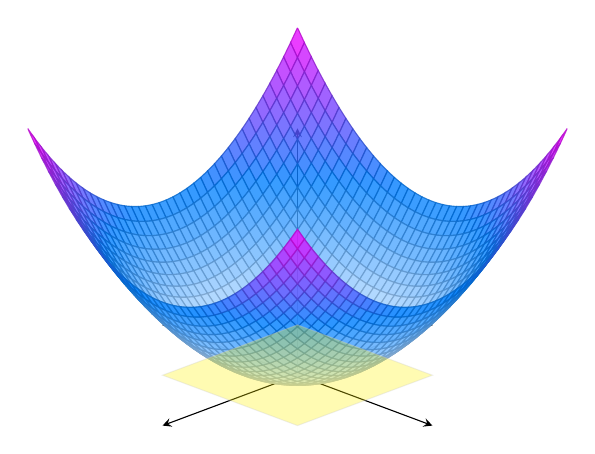
\begin{tikzpicture}
  \begin{axis}[
      view={135}{30},
      colormap/cool,
      axis lines=center,
      xlabel={}, ylabel={}, zlabel={},
      domain=-2:2,
      y domain=-2:2,
      samples=40,
      samples y=40,xtick=\empty,
ytick=\empty,
ztick=\empty
    ]

    % Paraboloid surface z = x^2 + y^2
    \addplot3[
      surf,
      opacity=0.8
    ]
    {x^2 + y^2};

    % Tangent plane at origin z = 0
    \addplot3 [
      surf,
      domain=-1:1,
      y domain=-1:1,
      samples=2,
      samples y=2,
      fill=yellow,
      opacity=0.3
    ]
    {0};

  
   

  \end{axis}
\end{tikzpicture}
    \caption{Notice how all the tangents at the lowest point of the paraboloid $(x=0,y=0)$ is constrained to be in the yellow coloured plane. Now only some area around $x=0,y=0$ can be made to look locally like the yellow plane and hence the definition of velocity will be valid only locally, within that patch.   }
\end{figure}
\subsection{Affine Connection}
Suppose in a locally inertial frame, for an object we have zero acceleration, that is:
$$\dv[2]{X^\alpha}{\uptau} = 0$$
Suppose the coordinates $X^\alpha \equiv X^\alpha(x^\mu)$ where $x^\mu$ are coordinates of a ground-based inertial reference frame relative to which the object accelerates. Then using chain rule, we have from the previous relation:
$$\frac{d}{d\uptau}\brac{\pdv{X^\alpha}{x^\mu}\dv{x^\mu}{\uptau}} = 0$$

Using product rule and chain rule again, we have:
$$\pdv{X^\alpha}{x^\mu}\dv[2]{x^\mu}{\uptau} +\pdv{X^\alpha}{x^\mu}{x^\rho} \dv{x^\rho}{\uptau} \dv{x^\mu}{\uptau}=0$$
Now we do one nice thing: multiply the above with $\pdv{x^\lambda}{X^\alpha}$:
$$\pdv{x^\lambda}{X^\alpha}\brac{\pdv{X^\alpha}{x^\mu}\dv[2]{x^\mu}{\uptau}} +\pdv{x^\lambda}{X^\alpha}\brac{\pdv{X^\alpha}{x^\mu}{x^\rho} \dv{x^\rho}{\uptau} \dv{x^\mu}{\uptau}}=0$$
Doing this, a nice thing occurs but for that we have to note that $\pdv{x^\lambda}{X^\alpha}\pdv{X^\alpha}{X^\mu} = \tensor{\delta}{^\lambda _\mu}$. Then from the first term, we get the kronecker delta and the expression reduces to:
$$\dv[2]{x^\lambda}{\uptau} +\mathcolor{blue}{\pdv{x^\lambda}{X^\alpha}\pdv{X^\alpha}{x^\mu}{x^\rho}} \dv{x^\rho}{\uptau} \dv{x^\mu}{\uptau}=0 \quad \implies \quad \dv[2]{x^\lambda}{\uptau} +\mathcolor{blue}{\tensor{\Gamma}{^\lambda _\mu _\rho}} \dv{x^\rho}{\uptau} \dv{x^\mu}{\uptau}=0$$
Here we have identified the scary blue term with a symbol with three indices, one upper and two lower (since in the blue term, there is one upper and two lower indices). This thing, we call the \textbf{affine connection}. 
Note that since derivatives commute\footnote{If a space has something called a `torsion', then the derivatives no longer commute and the following property does not hold true} generally, we have the lower indices of the affine connection to be symmetric, that is,
$$\tensor{\Gamma}{^\alpha _\mu _\nu} =\tensor{\Gamma}{^\alpha _\nu _\mu}$$
\subsubsection{Transformation of Affine Connection}
Note that the affine connection contains both coordinates $X^\alpha$ and $x\mu$. Suppose we want to transform from $x$ to $x'$ coordinate system, then only the $x$ things will be changed, not the $X$ things. Leave the $X$ alone. Anyways, the $X^\alpha$ is getting summed over, so put primes only on the indices which remain finally. So we have:
\begin{align*}
    \tensor{(\Gamma')}{^\lambda _\mu _\nu} &= \mathcolor{blue}{\pdv{x'^\lambda}{X^\alpha}}\pdv{X^\alpha}{x'^\mu}{x'^\nu}\\
    &= \mathcolor{blue}{\pdv{x'^\lambda}{x^\rho}\pdv{x^\rho}{X^\alpha}}\pdv{X^\alpha}{x'^\mu}{x'^\nu} \quad \text{(using chain rule )}\\
    &=\brac{\pdv{x'^\lambda}{x^\rho}\pdv{x^\rho}{X^\alpha}} \pdv{x'^\mu}\brac{\mathcolor{OliveGreen}{\pdv{X^\alpha}{x^\sigma}}\mathcolor{red}{ \pdv{x^\sigma}{x'^\nu}}} \quad \text{(using chain rule again )}\\
    &=\brac{\pdv{x'^\lambda}{x^\rho}\pdv{x^\rho}{X^\alpha}}\brac{ { \mathcolor{red}{\pdv{x^\sigma}{x'^\nu}}\pdv{x'^\mu}\brac{\mathcolor{OliveGreen}{\pdv{X^\alpha}{x^\sigma}}} + \mathcolor{OliveGreen}{\pdv{X^\alpha}{x^\sigma}}\pdv{\mathcolor{red}{x^\sigma}}{x'^\mu}{\mathcolor{red}{x'^\nu}}}}\quad \text{(using product rule )}\\
    &=\brac{\pdv{x'^\lambda}{x^\rho}\pdv{x^\rho}{X^\alpha}} \brac{\pdv{x^\sigma}{x'^\nu} \pdv{X^\alpha}{x^\kappa}{x^\sigma}\pdv{x^\kappa}{x'^\mu}+ \pdv{X^\alpha}{x^\sigma}\pdv{x^\sigma}{x'^\mu}{x'^\nu}}\quad \text{(using chain rule )}
\end{align*}
Well well, I know this was a shitty calculation but hey, sometimes shit is what relieves us! We now focus on the two terms separately in the above expression. 
\begin{itemize}
    \item \textbf{The First Term:} $\brac{\pdv{x'^\lambda}{x^\rho}\pdv{x^\rho}{X^\alpha}}\pdv{x^\sigma}{x'^\nu} \pdv{X^\alpha}{x^\kappa}{x^\sigma}\pdv{x^\kappa}{x'^\mu}$\\[0.3cm]
This can be rearranged a bit and can be written as 
$$   \brac{\pdv{x'^\lambda}{x^\rho}\pdv{x^\sigma}{x'^\nu} \pdv{x^\kappa}{x'^\mu}}   \brac{\pdv{x^\rho}{X^\alpha}\pdv{X^\alpha}{x^\kappa}{x^\sigma}} \equiv \brac{\pdv{x'^\lambda}{x^\rho}\pdv{x^\sigma}{x'^\nu} \pdv{x^\kappa}{x'^\mu}}  \tensor{\Gamma}{^\rho _\kappa _\sigma}$$
\item \textbf{The Second Term:} $\brac{\pdv{x'^\lambda}{x^\rho}\mathcolor{blue}{\pdv{x^\rho}{X^\alpha}}}\mathcolor{blue}{\pdv{X^\alpha}{x^\sigma}}\pdv{x^\sigma}{x'^\mu}{x'^\nu}$
The blue terms together gives $\tensor{\delta}{^\rho _\sigma}$ which reduces the expression to:
$$\pdv{x'^\lambda}{x^\rho}\pdv{x^\rho}{x'^\mu}{x'^\nu}$$
\end{itemize}
Thus, finally we obtain the expression for the transformation of the affine connection:
$$\boxed{ \tensor{(\Gamma')}{^\lambda _\mu _\nu} = \brac{\pdv{x'^\lambda}{x^\rho}\pdv{x^\sigma}{x'^\nu} \pdv{x^\kappa}{x'^\mu}}  \tensor{\Gamma}{^\rho _\kappa _\sigma} +\pdv{x'^\lambda}{x^\rho}\pdv{x^\rho}{x'^\mu}{x'^\nu} }$$
Note that the first term is the usual transformation rule for the affine connection but again the second BAD term emerges which, if non-zero, will lead to the affine connection not being a tensor.\\[0.3cm]
Now note that the BAD term contains the second derivative of the old coordinates with respect to the old coordinates, but generally we have the other way. So it would be a bit nice if we could change it. For that, note the identity and differentiate with respect to $x'^\mu$:
\begin{align*}
   &\pdv{x'^\lambda}{x^\rho}\pdv{x^\rho}{x'^\nu}=\tensor{\delta}{^\lambda_\nu}\\
\implies & \pdv{x'^\mu}\brac{\pdv{x'^\lambda}{x^\rho}\pdv{x^\rho}{x'^\nu}}=0\\
\implies & \brac{\pdv{x'^\lambda}{x^\rho}} \brac{\pdv{x^\rho}{x'^\nu}{x'^\mu} }+ \brac{\pdv{x^\rho}{x'^\nu}}\brac{\pdv{x'^\lambda}{x^\rho}{x'^\mu}}=0\\
\implies & \brac{\pdv{x'^\lambda}{x^\rho}} \brac{\pdv{x^\rho}{x'^\nu}{x'^\mu} } + \brac{\pdv{x^\rho}{x'^\nu}}\brac{\pdv{x'^\lambda}{x^\rho}{x^\sigma}\pdv{x^\sigma}{x'^\mu}}=0
\end{align*}
The first term in the above is exactly the BAD term in the affine connection transformation and thus we replace this. Then we have: 
$$\boxed{ \tensor{(\Gamma')}{^\lambda _\mu _\nu} = \brac{\pdv{x'^\lambda}{x^\rho}\pdv{x^\sigma}{x'^\nu} \pdv{x^\kappa}{x'^\mu}}  \tensor{\Gamma}{^\rho _\kappa _\sigma} - \brac{\pdv{x^\rho}{x'^\nu}}\brac{\pdv{x'^\lambda}{x^\rho}{x^\sigma}\pdv{x^\sigma}{x'^\mu}} }$$
\subsection{Covariant Derivatives}
In every transformation seen so far, we had got a BAD term (containing a second derivative) which spoils the transformation. So wouldn't it be nice if we just redefine the definition of a derivative so that this BAD term gets cancelled from the definition only? This brings us to \textit{covariant derivative} 
\\[0.3cm]
\textbf{A Notational Nightmare:}
The symbol of covariant derivative is very confusing. Different people use different notation for it. Some use $D$ for it, some use $\nabla$ while some use $;$. We will use $;$ for it, I guess...\\[0.3cm]
The covariant derivative of a vector component with respect to a coordinate is defined as \footnote{$\tensor{A}{^\nu _, _\mu}$ means the normal derivative, that is, $\partial_\mu A^\nu$}: 
$$\tensor{A}{^\lambda _; _\mu} :=  \tensor{A}{^\lambda _, _\mu} +\tensor{\Gamma}{^\lambda _\mu _\nu}A^\nu$$
\subsection{Relating metric and affine connection}
\subsection{Curls, divergences and other craps}